\documentclass{../local}
\begin{document}

\section{REXOS Overall Architecture}
% How we changed the architecture, and why we made which decisions
This is the second iteration of the REXOS architecture. Figure 1 shows a overview of all system components.
\begin{center}
	\begin{figure}[h!]
		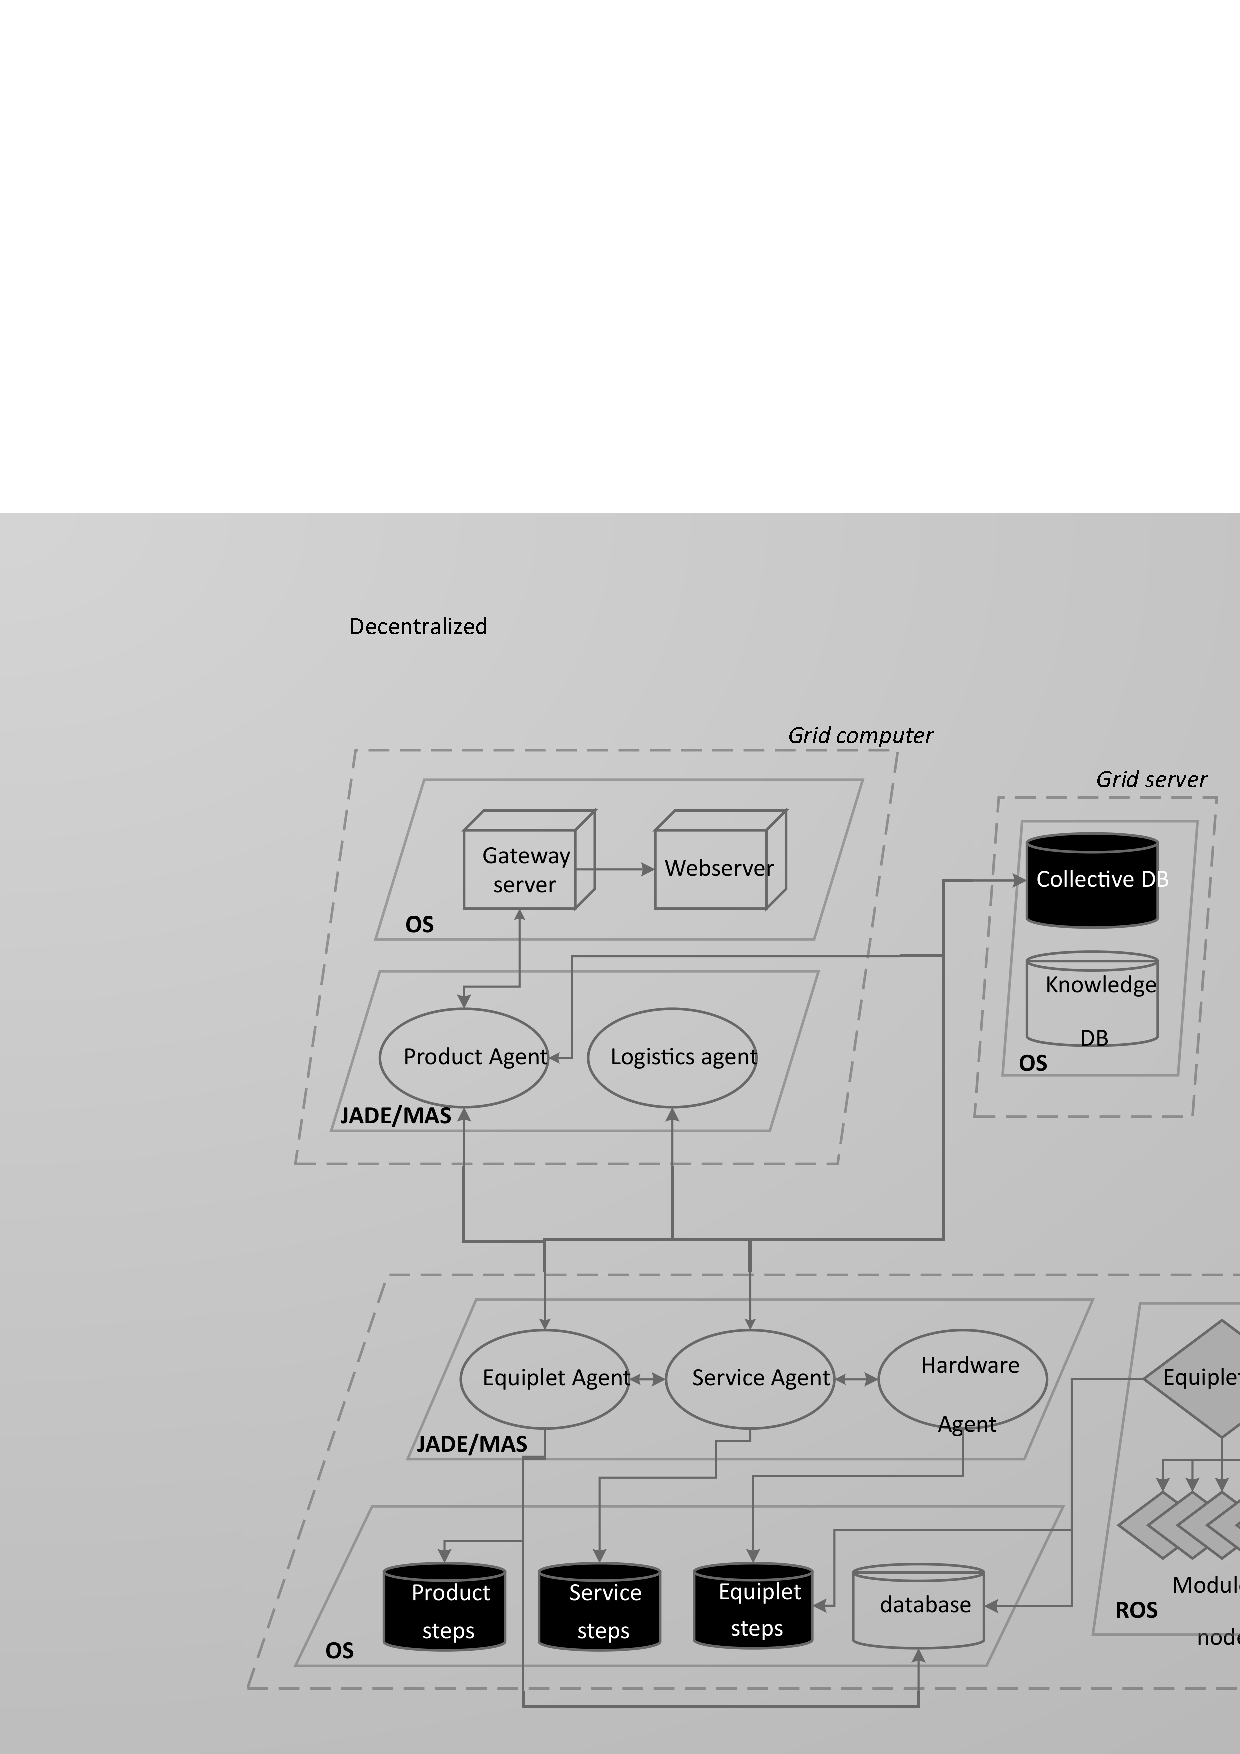
\includegraphics[width=17cm]{../images/Decentralized_REXOS.jpg}
		\centering
		\caption{Current load of equiplets - Heterarchical}
	\end{figure}
	\label{fig:systemOverView}
\end{center}

%It was designed to give a draw demo, which was far below requirements. The 'mainframe' of the architecture was present, but poorly implemented and documented.
%The current system houses 2 major components. MAS, which represents the intellegent part of the system, and ROS, the part responsible for executing commands.

The first iteration of the REXOS architecture was not fully implemented. The major components of the architecture where present, but poorly implemented and barely documented. The architecture houses 2 major components known as layers. These layers are the MAS layer, which represents the intelligent part of the system, and ROS, the part responsible for controlling the hardware.

\subsection{MAS}
%Tell smth about implementation of the curr MAS system, what purpose it serves, and how its implemented.%
The MAS\footnote{Multi agent system. See abbreviations for more detail.} was designed to be the intelligent and cognitive side of the REXOS platform. It incorperates virtual autonomous entities known as agents and is implemented in JADE \textbf{ref2section}. As shown in figure ~ \ref{systemOverView} 5 agents are present. The MAS also provides needed product abstraction. Product abstraction is implemented to provide a means to tranform a physical product in low level hardware instructions. Reasearchers in the 2012 - 2013 research semester implemented this product abstraction.\footnote{for more information see; \emph{Product Abstraction for Reconfigurable Manufacturing Systems} }

\begin{description}
  \item[Product agent] \hfill \\
		The product agents is a virtual representation of the product. It is responsible for scheduling itself with the equiplets it need for finishing the product. The product agent will always communicate with the equiplet agent in order to complete its product steps. The product agent that was implemented lacked a proper scheduling algorithm.
  \item[Equiplet agent] \hfill \\
  The equiplet agent represents a equiplet. The equiplet agent is responsible for all communication with the product agent. It is responsbile for its own schedule. It communicates with its service agent in order to translate the different steps needed to perform product abstraction.
  \item[Service agent] \hfill \\
  		The service agent handles all service level translations.It communicates with the hardware agent and equiplet agent to perform translation of steps. The service agent is responsible for managing services offered by the equiplet. Because the initial services are fairly generic, not much needed to be changed.  
  \item[Hardware agent] \hfill \\
  The harware agent represents the different hardware modules present on the equiplet. The hardware agent is responsible for 'controlling' the hardware. It also handles module step translations. The hardware agent is the only agent that 'communicates' with ROS.
  \item[Logistics agent] \hfill \\
  		The logistics handles all logistic operations and data within the grid. It is responsible for reporting logistic information to the entities in the grid. The logistics agent communicates with the product agent to report transport times \& part information. 
  		product agent communication
\end{description}

\subsubsection{Knowledge database}
The current knowledge database is implemented in the previous iteration. They implemented the knowledge database in order to facilitate product abstraction and to provide a central place where data is stored. All information about parts, equiplets, services and modules are stored in the knowledge database.

\subsubsection{Modules}
In this implementation of the MAS, only 1 module was implemented due to time constraints. Modules in MAS provide the code needed to translate service steps into hardware steps. Modules are used by the service agent. In the current implementation of the MAS, only the delta robot module and the pen module where implemented.

\subsection{Inter-layer communication}
Communication between the ROS and MAS layers is an important aspect of REXOS. Communication is defined in distinct ways. All data exchange happens through blackboards. A blackboard is used to transport data. The difference between a blackboard and a normal data-channel is that blackboard provide ways to seperate read and write permissions. This means that blackboards can be configured to allow for one entity to read and write from it, whilst the other is only allowed to write on it. Communication between agents all happends through the JADE's own communication system, called acl messages\footnote{http://jade.cselt.it/doc/api/jade/lang/acl/ACLMessage.html}.
\begin{center}
	\includegraphics[width=15cm]{../images/REXOSCommunicationDiagram.png}
	\captionof{figure}{REXOS communication diagram (taken from \emph{[Design] REXOS Basic Architecture}) }
\end{center}

\subsection{ROS}
%Tell smth about implementation of the curr ROS system, what purpose it serves, and how its implemented.%
The ROS layer represents all the hardware. All ROS actions are non-autonomous and driven by the intelligent side of REXOS. This means that all MAS-Agents take smart and cognitive decisions and ROS executes these. 

\subsubsection{Ros Nodes}
The ROS-layer consists of nodes. Nodes are software entities responsible for handling a specific task. In REXOS Ros nodes represent modules. The ROS node representing the equiplet is called the equiplet node. All ROS node's are independent and should be able to operate autonomously.

\subsubsection*{Equiplet node}
The equiplet node is responsible for controlling all modules on the ROS side. The equiplet node consists of a single ROS node. All modules attached to the equiplet (ROS nodes aswell) are registered at the equiplet node. This is implemented to allow sending of instructions and updating of states throughout all the modules. The equiplet node is designed as to only allow instructions that are tailor made for drawing (i.e. using the delta robot module with the pen module).

\subsubsection*{Delta robot node}
They delta robot node is responsible for providing ways to manage the delta robot module that can be attached to equiplets. Currently the delta robot module doesnt allow for dynamic coordinates that the new vision system uses. The initial delta robot module is written for use with the pen-module because of which the delta robot module needs an overhaul to function with the rest of the system.

\subsubsection{MAST}
% The initial state of MAST
MAST is an abbreviation for MAchine STates and is used for representing the state of the equiplets. The safety and abilities of the equiplets depend on their internal state. In RMS, having actuators activate when it is not expected can cause harm to people and damage to the surroundings, for that reason, MAST was developed. MAST will insure that an actuator is not activated when it is no expected. It does this using the following model:

\begin{center}
	\includegraphics[width=6cm]{../images/MAST.png}
	\captionof{figure}{The seven states of MAST}
\end{center}

The safe, standby and normal state are active states. The setup, shutdown, start and stop states are transition states. For an entity (equiplet or module) to reach a new active state, it has to successfully traverse the transitional state that precedes it. MAST is setup in such a way that the combined state of all the modules on an equiplet is equal to the highest (furthest from safe) state of any of the modules. This means that if even one module is not in a safe state, the whole equiplet is not safe.

\subsubsection{Vision}
In previous iterations of REXOS vision was a big obstacle. Since all equiplets operate on a cheap camera, optimised vision algorithms are of key importance. The vision library was virtually non-existent and poorly documented. 

\end{document}